\chapter{Example Video Coding Manual} \label{app:codingmanual}
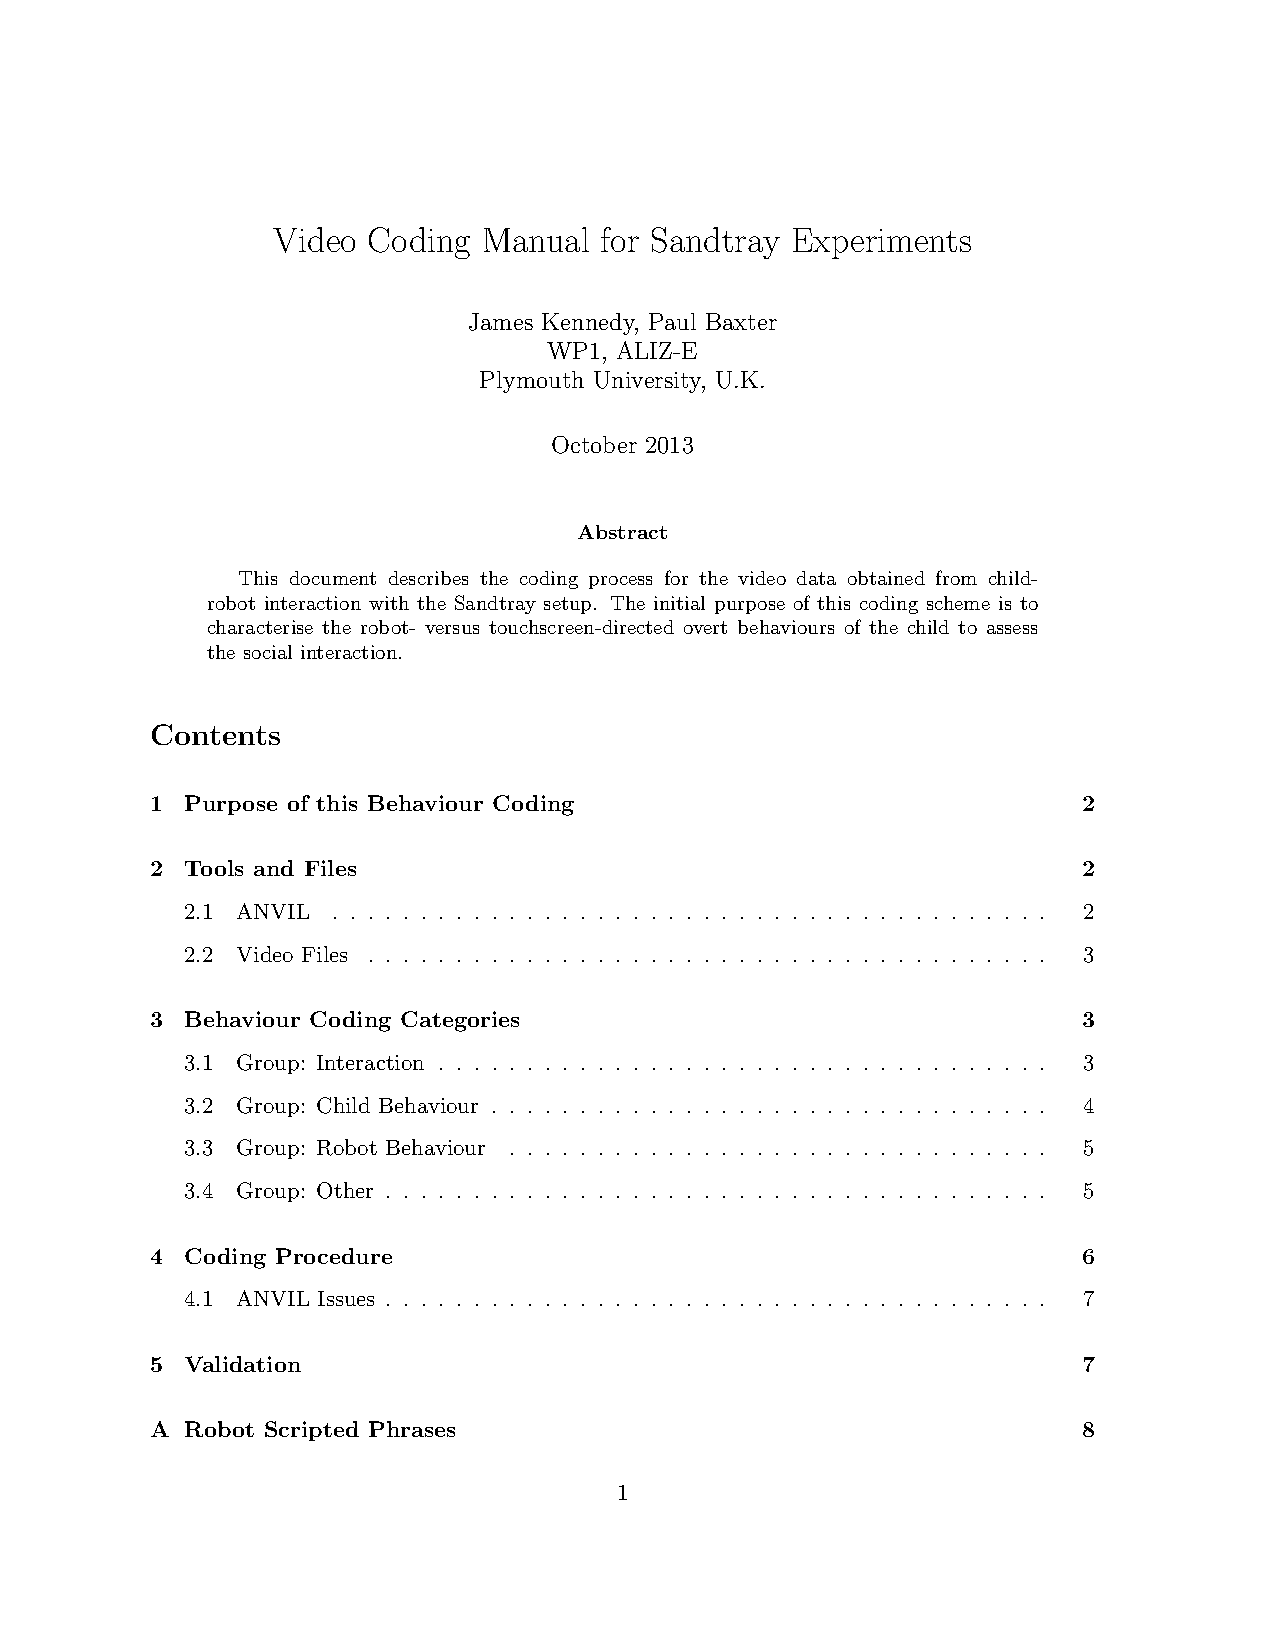
\includepdf[pages=1-8,pagecommand={},linktodoc=true]{appendices/CodingManual.pdf}

\cleartooddpage
\chapter{Crowdsourced Immediacy Results} \label{app:crowdsourced}
Below is the table of data collected as described in Chapter \ref{chap:method}, from adults rating the robot behaviour in several of the experimental conditions.

\begin{table}[h!]
	\centering
	\caption{Adult crowdsourced nonverbal immediacy ratings for robot behaviours, including the chapter that the behaviour is evaluated in, and basic demographic details.}
	\label{tab:app-crowdsource}
	\renewcommand{\arraystretch}{1.2} 
	\begin{tabular}{@{}clccll@{}}
	\toprule
	\textbf{Chapter}	& \textbf{Condition}	& \textbf{Adult \textit{N}}	& \textbf{Age \textit{M} (\textit{SD})} & \textbf{Gender} & \begin{tabular}[t]{@{}l@{}}\textbf{NVI Score}\\ \textbf{\textit{M} (\textit{95\%CI})}\end{tabular} \\ \midrule
	\ref{chap:embodiment} 	& `Real' robot		& 37 & 35.8 (\textit{13.2}) & 24M/13F & 51.9 (\textit{50.5,53.3})\\
	\ref{chap:embodiment} 	& `Virtual' robot	& 35 & 35.6 (\textit{13.1}) & 20M/15F & 50.2 (\textit{48.5,51.9})\\
	\ref{chap:socasoc} 		& Social robot		& 33 & 29.0 (\textit{10.4}) & 21M/12F & 49.0 (\textit{47.6,50.4})\\
	\ref{chap:socasoc} 		& Asocial robot		& 30 & 39.0 (\textit{12.2}) & 14M/16F & 48.5 (\textit{46.1,50.8})\\	
	\ref{chap:nviexperiment} & Low NVI robot	& 33 & 31.5 (\textit{12.2}) & 19M/14F & 40.2 (\textit{38.1,42.2})\\
	\ref{chap:nviexperiment} & High NVI robot	& 31 & 35.6 (\textit{11.7}) & 18M/13F & 48.4 (\textit{46.9,50.0})\\
	\ref{chap:behavemodel}	& Human				& 30 & 32.9 (\textit{12.3}) & 18M/12F & 47.7 (\textit{45.3,50.1})\\ \bottomrule
	\end{tabular}
\end{table}

\cleartooddpage
\chapter{Chapter \ref{chap:validation} Short Story Script} \label{app:story}
The following is the short story script as used in Chapter \ref{chap:validation}. The story is largely based on one from the following website: \href{http://freestoriesforkids.com/children/stories-and-tales/robot-virus}{http://freestoriesforkids.com/children/stories-and-tales/robot-virus} (produced here with permission from the author).

\textit{Hello, I'm Charlie. Today I'm going to tell you one of my favourite robot stories. It is about a boy, his name is Ricky, and his robot helper, Johnny. Ricky lived in a lovely futuristic house, which had everything you could ever want. Though he didn't help much around the house, Ricky was still as pleased as punch when his parents bought him the latest model of helper robot. As soon as it arrived, off it went; cooking, cleaning, ironing, and - most importantly - gathering up old clothes from Ricky's bedroom floor, which Ricky didn't like having to walk on.}

\textit{On that first day, when Ricky went to sleep, he had left his bedroom in a truly disastrous state. When he woke up the next morning, everything was perfectly clean and tidy. In fact, it was actually too clean. Ricky could not find his favourite blue skateboard. However much he searched, it did not reappear, and the same was starting to happen with other things. Ricky looked with suspicion at the gleaming helper robot. He hatched a plan to spy on the robot, and began following it around the house. }

\textit{Finally he caught it red-handed. It was picking up a toy to hide it. Off he went, running to his parents, to tell them that the helper was broken and badly programmed. Ricky asked them to have it changed. But his parents said absolutely not; it was impossible, they were delighted with the new helper, and that it was the best cleaner they had ever met. So Ricky needed to get some kind of proof; maybe take some hidden photos. He kept nagging his parents for 3 whole weeks about how much good stuff the robot was hiding. Ricky argued that this was not worth the clean house because toys are more important.}

\textit{One day the robot was whirring past, and heard the boy's complaints. The robot returned with five of his toys, and some clothes for him.``Here sire, I did not know it was bothering you'', said the helper, with its metallic voice. ``How could it not you thief?! You've been nicking my stuff for weeks'', the boy answered, furiously. The robot replied, ``the objects were left on the floor. I therefore calculated that you did  not like them. I am programmed to collect all that is not wanted, and at night I send it to places other humans can use it. I am a maximum efficiency machine. Did you not know?''.}

\textit{Ricky started feeling ashamed. He had spent all his life treating things as though they were useless. He looked after nothing. Yet it was true that many other people would be delighted to treat those things with all the care in the world. And he understood that the robot was neither broken nor badly programmed, rather, it had been programmed extremely well! Since then, Ricky decided to become a Maximum Efficiency Boy, and he put real care into how he treated his things. He kept them tidy, and made sure that he didn't have more than was necessary. And, often, he would buy things, and take them along with his good friend, the robot, to help out those other people who needed them.}

\textit{The end... I hope you enjoyed the story. Goodbye!}

\cleartooddpage
\chapter{Chapter \ref{chap:validation} Short Story Recall Questionnaire} \label{app:story_questions}
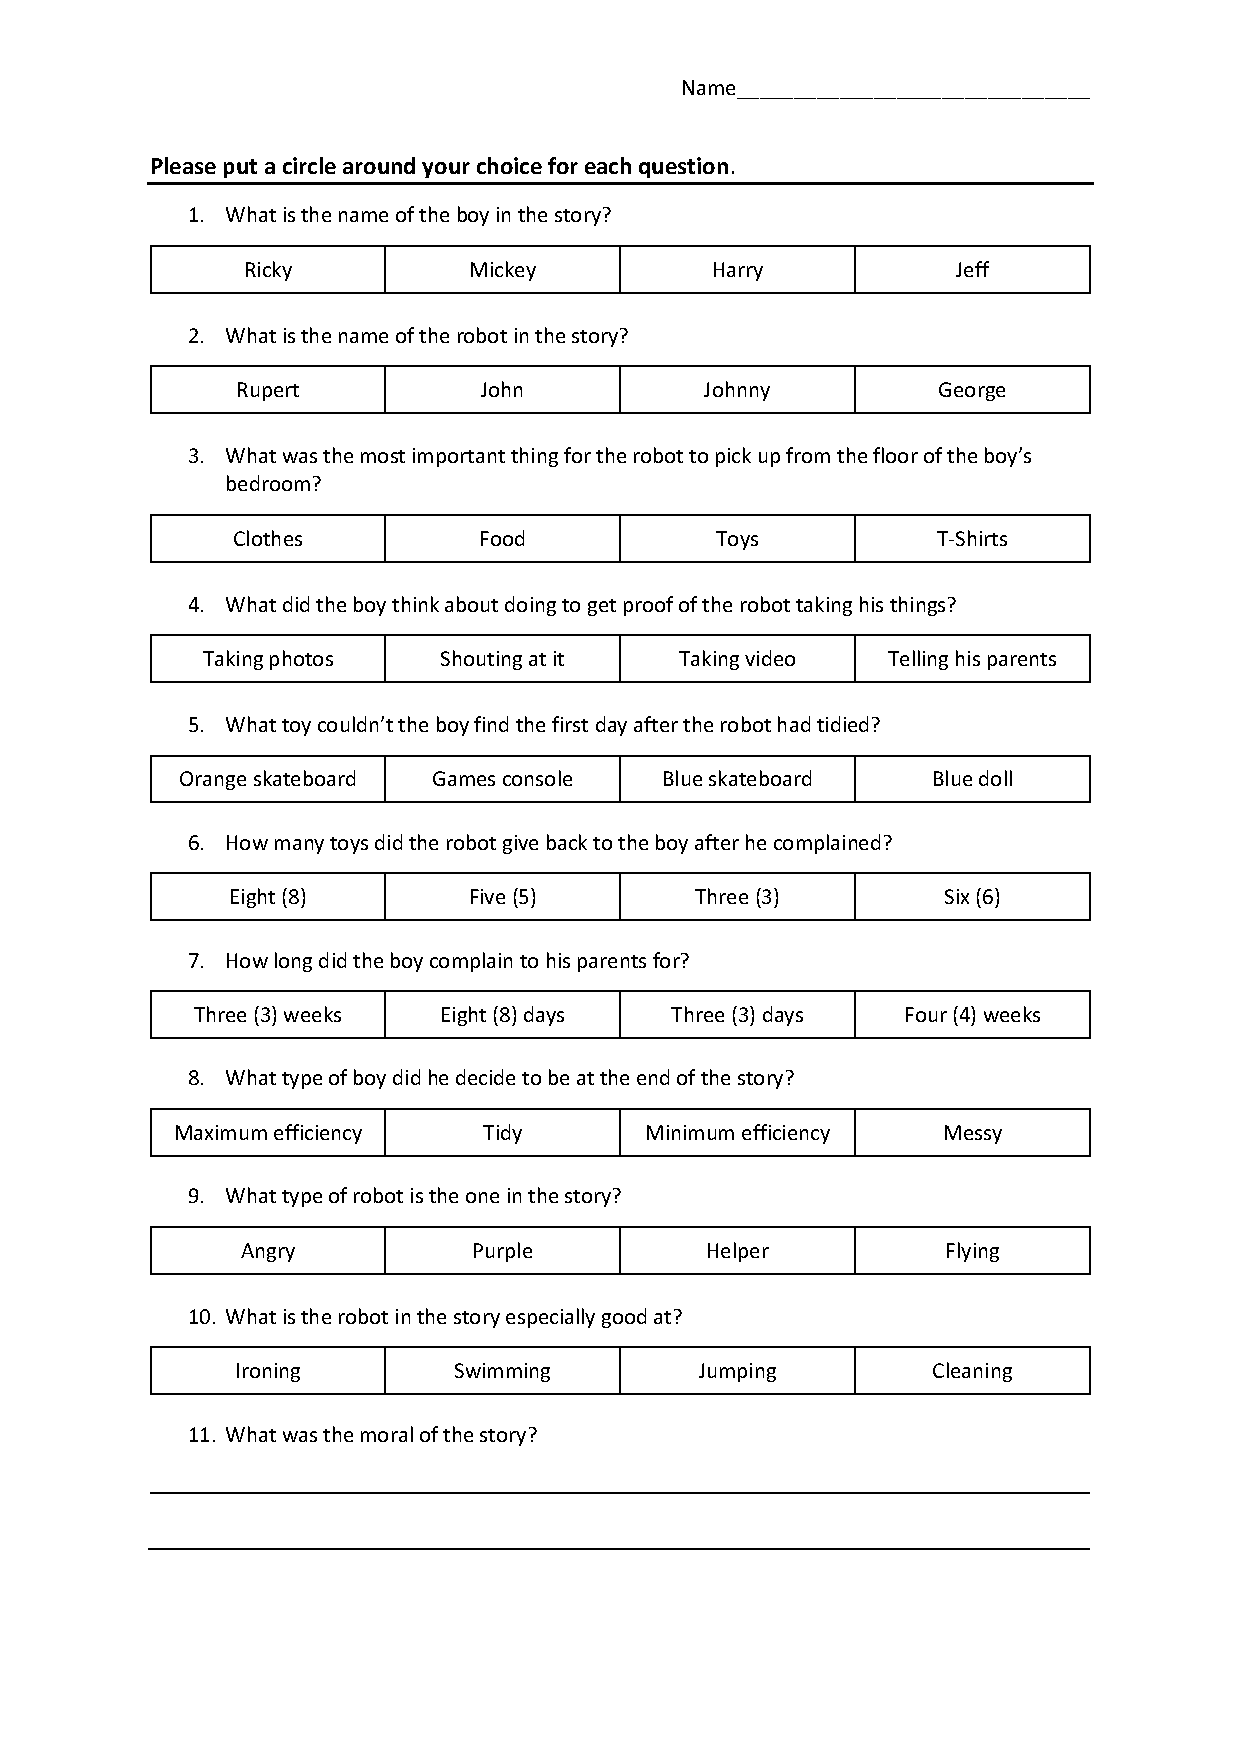
\includepdf[pages=1,pagecommand={},linktodoc=true]{appendices/ch4_Story_Questions.pdf}

\cleartooddpage
\chapter{Robot Nonverbal Immediacy Questionnaire} \label{app:rniq}
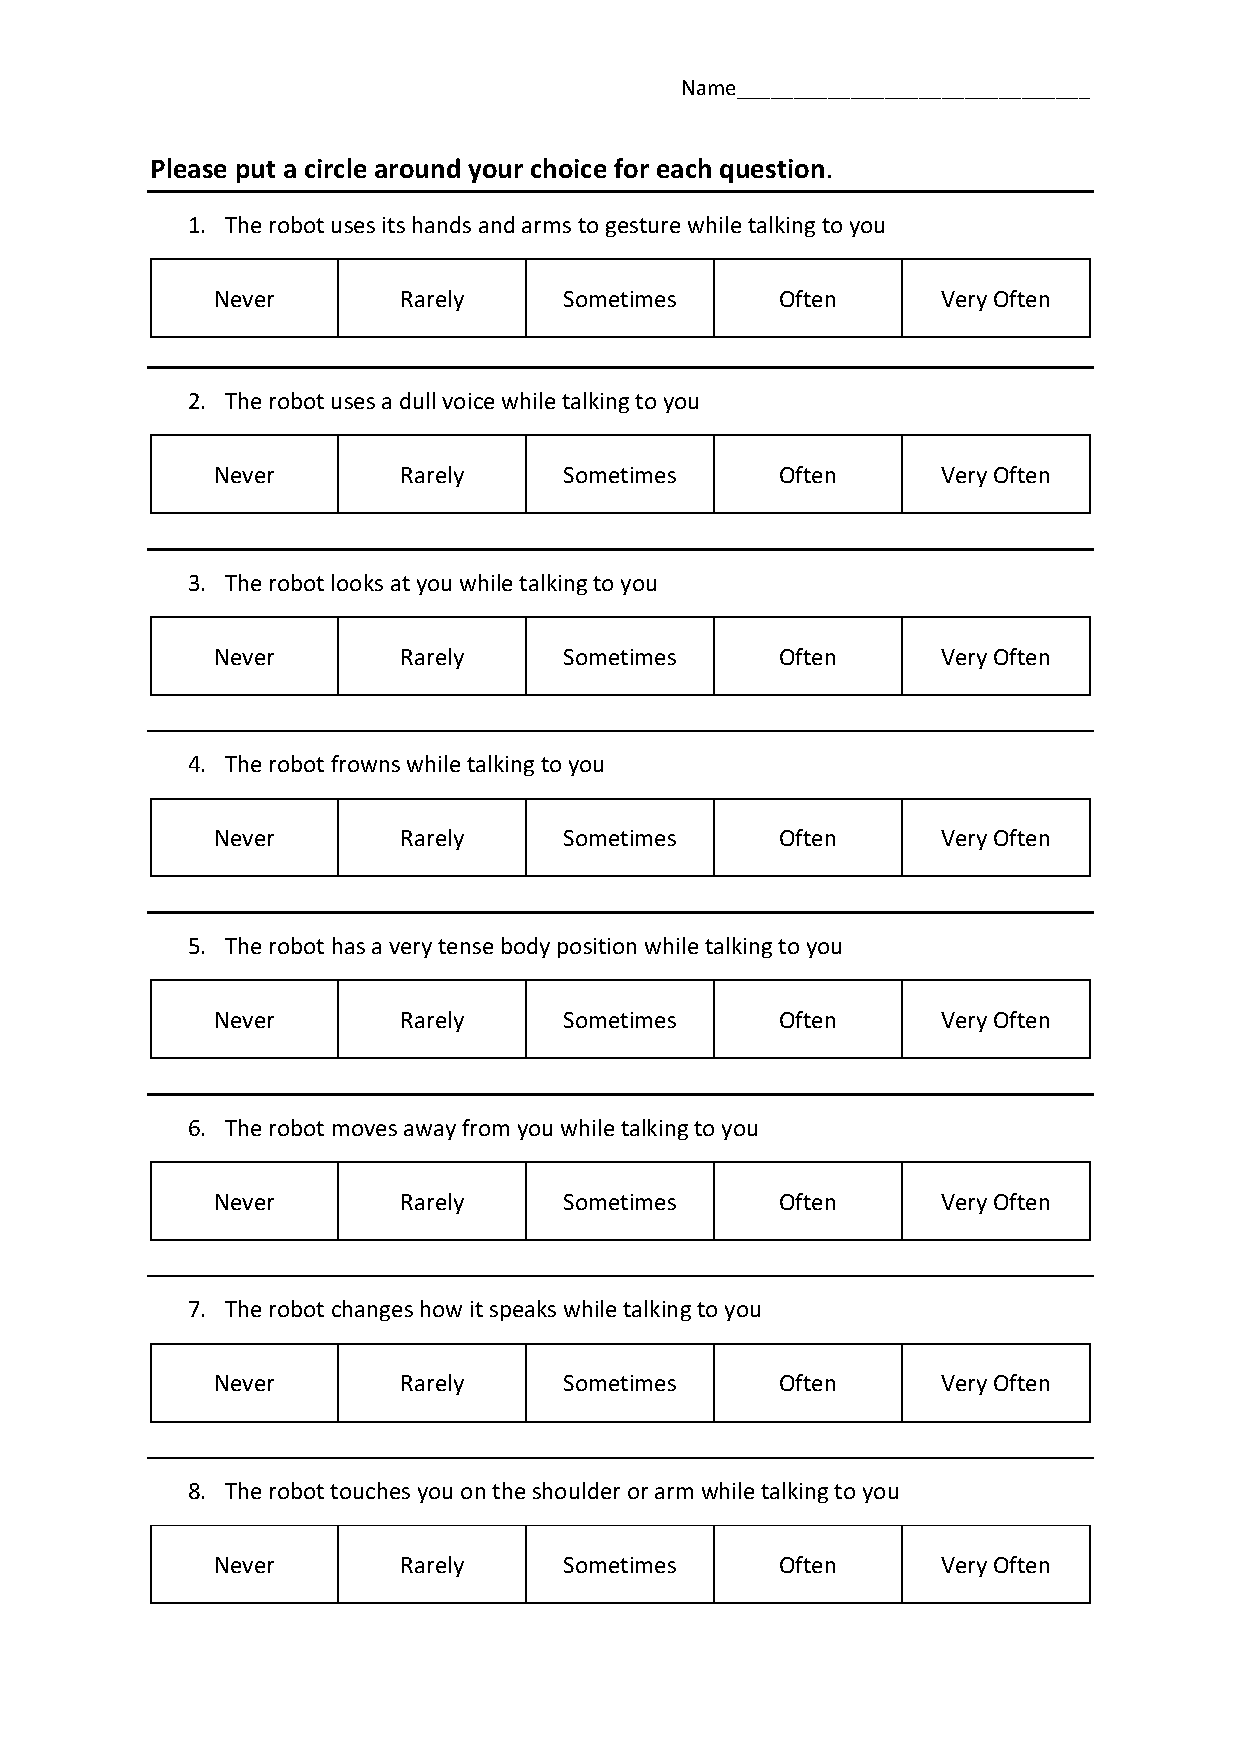
\includepdf[pages=1-2,pagecommand={},linktodoc=true]{appendices/RNIQ.pdf}

\cleartooddpage
\chapter{Child Nonverbal Immediacy Questionnaire} \label{app:cniq}
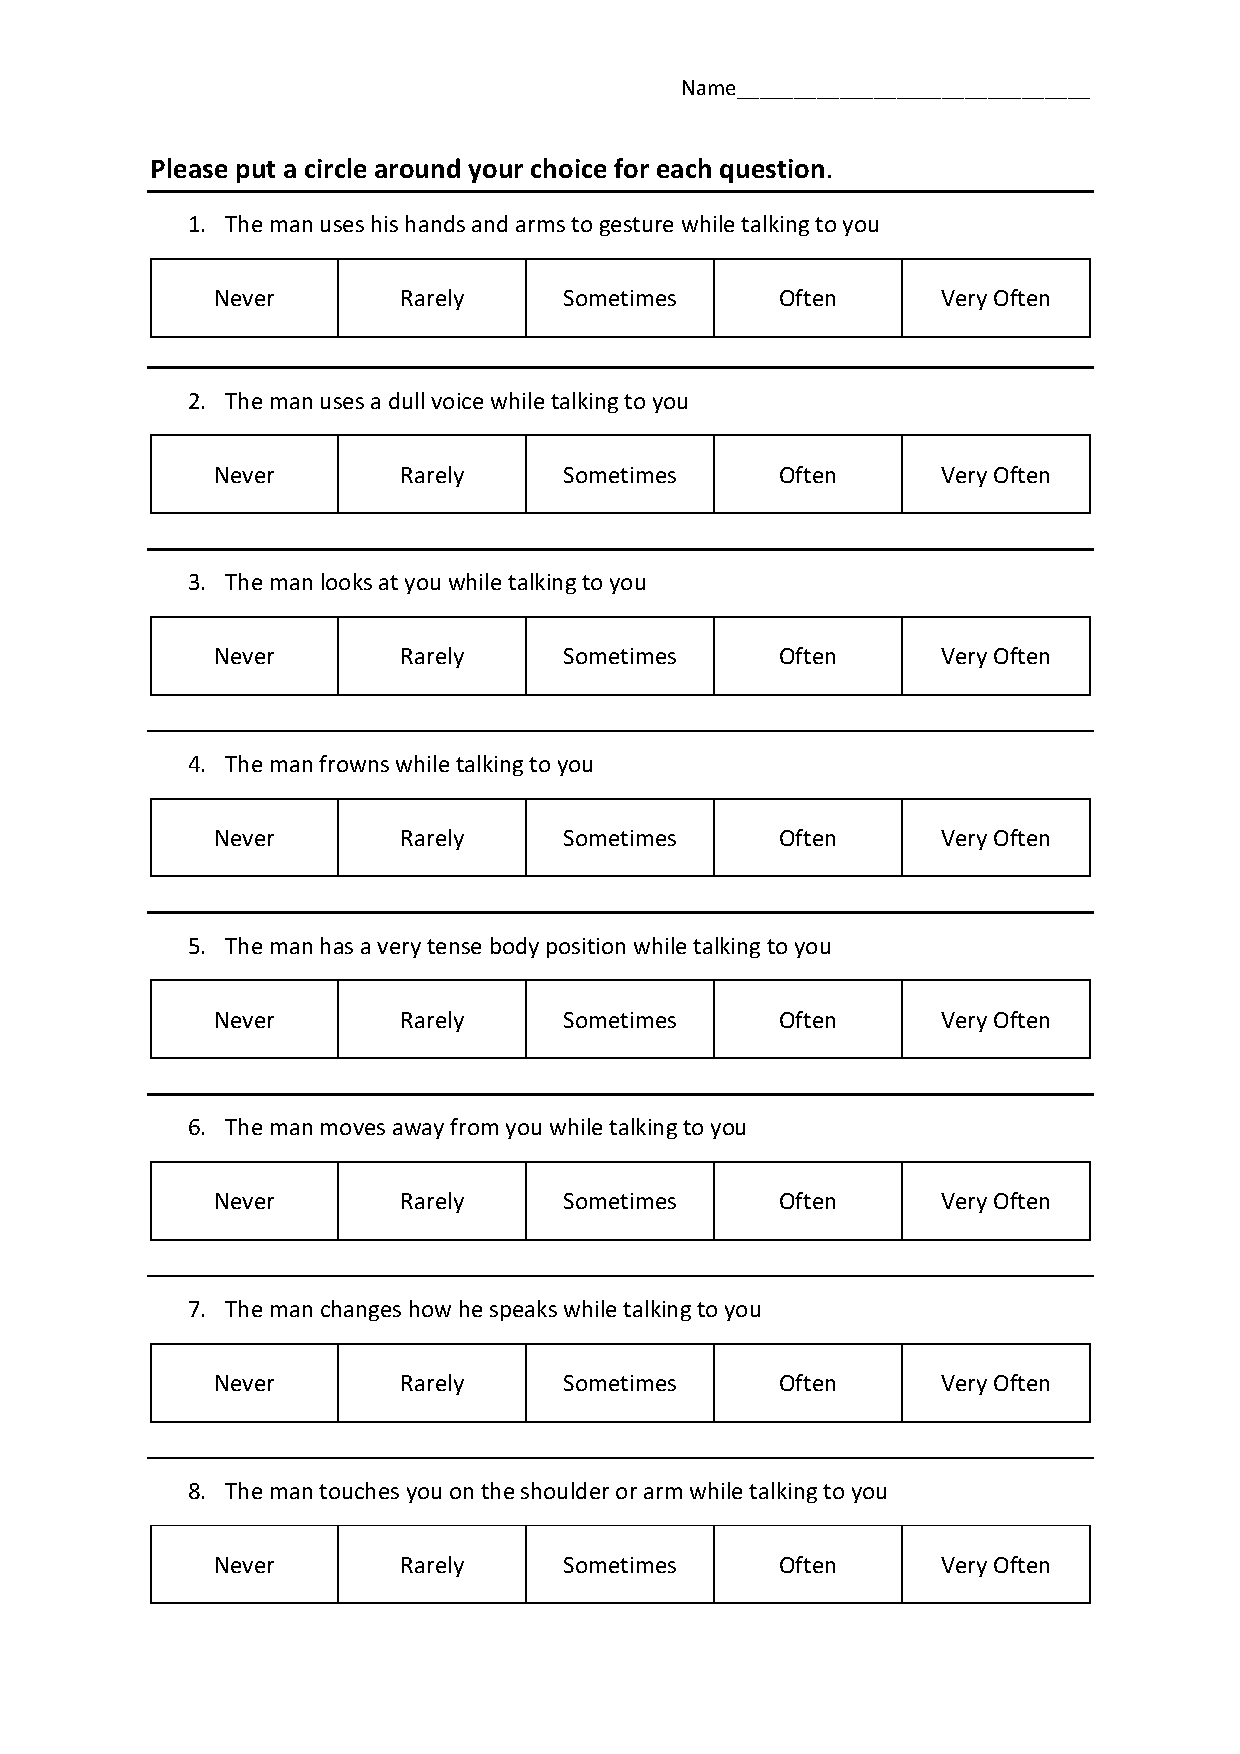
\includepdf[pages=1-2,pagecommand={},linktodoc=true]{appendices/CNIQ.pdf}

\cleartooddpage
\chapter{Chapter \ref{chap:embodiment} Robot Script} \label{app:ch6-robotscript}
\textbf{Robot Instructions}

\textit{"Hello! I'm Pop/Crackle. Right, what we are going to be doing today is sorting out some aliens. We have two species of aliens that are lost in space and we have to return them to their home planet. Okay? So here we have our different types of aliens and our two planets, the purple and the orange. We need to sort them into their two different groups. I'd like you to see if you can guess which planets the aliens are from. You can touch an alien and you drag it to the planet you think it's from, and it'll tell you whether you are right or not. I won't help you on your first go. Let's see how well you can do on your own! Now you can start."}

\textbf{Prior to Guided Discovery Phase}

\textit{"Lovely, well done. Now I'll give you a clue, the aliens from the purple planet all have something in common."}

\textbf{Prior to Post-Test}

\textit{"Right, we'll do just one more set of aliens. Using the practice we've just done, let's see how well you can do. I won't help you this time. Have a go."}

\textbf{Robot Goodbye}

\textit{"Well done. thank you very much. Thank you for helping me out today. You can go back to your class. Goodbye!"}

\cleartooddpage
\chapter{Robot Immediacy Questionnaire} \label{app:riq}
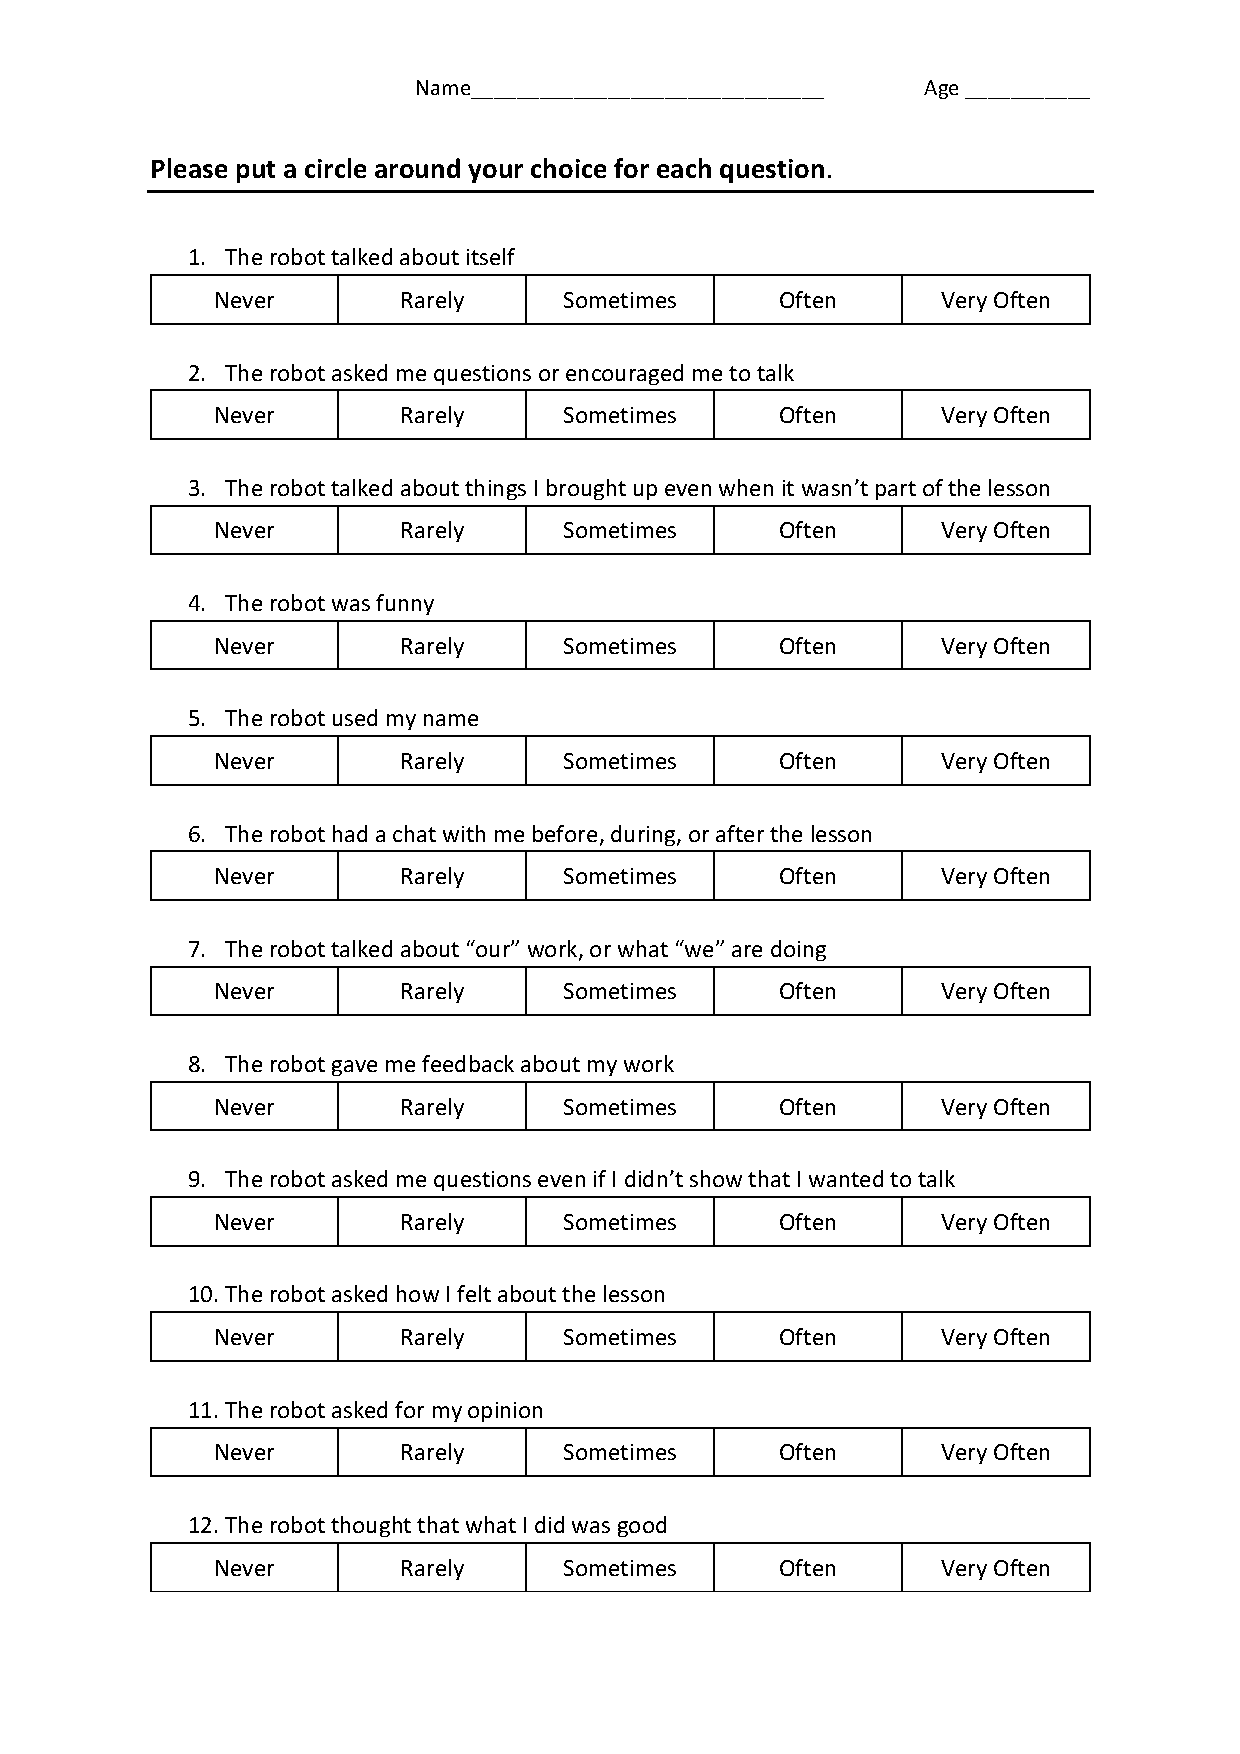
\includepdf[pages=1-2,pagecommand={},linktodoc=true]{appendices/RIQ.pdf}

\cleartooddpage
\chapter{Robot Relationship Questionnaire} \label{app:rrq}
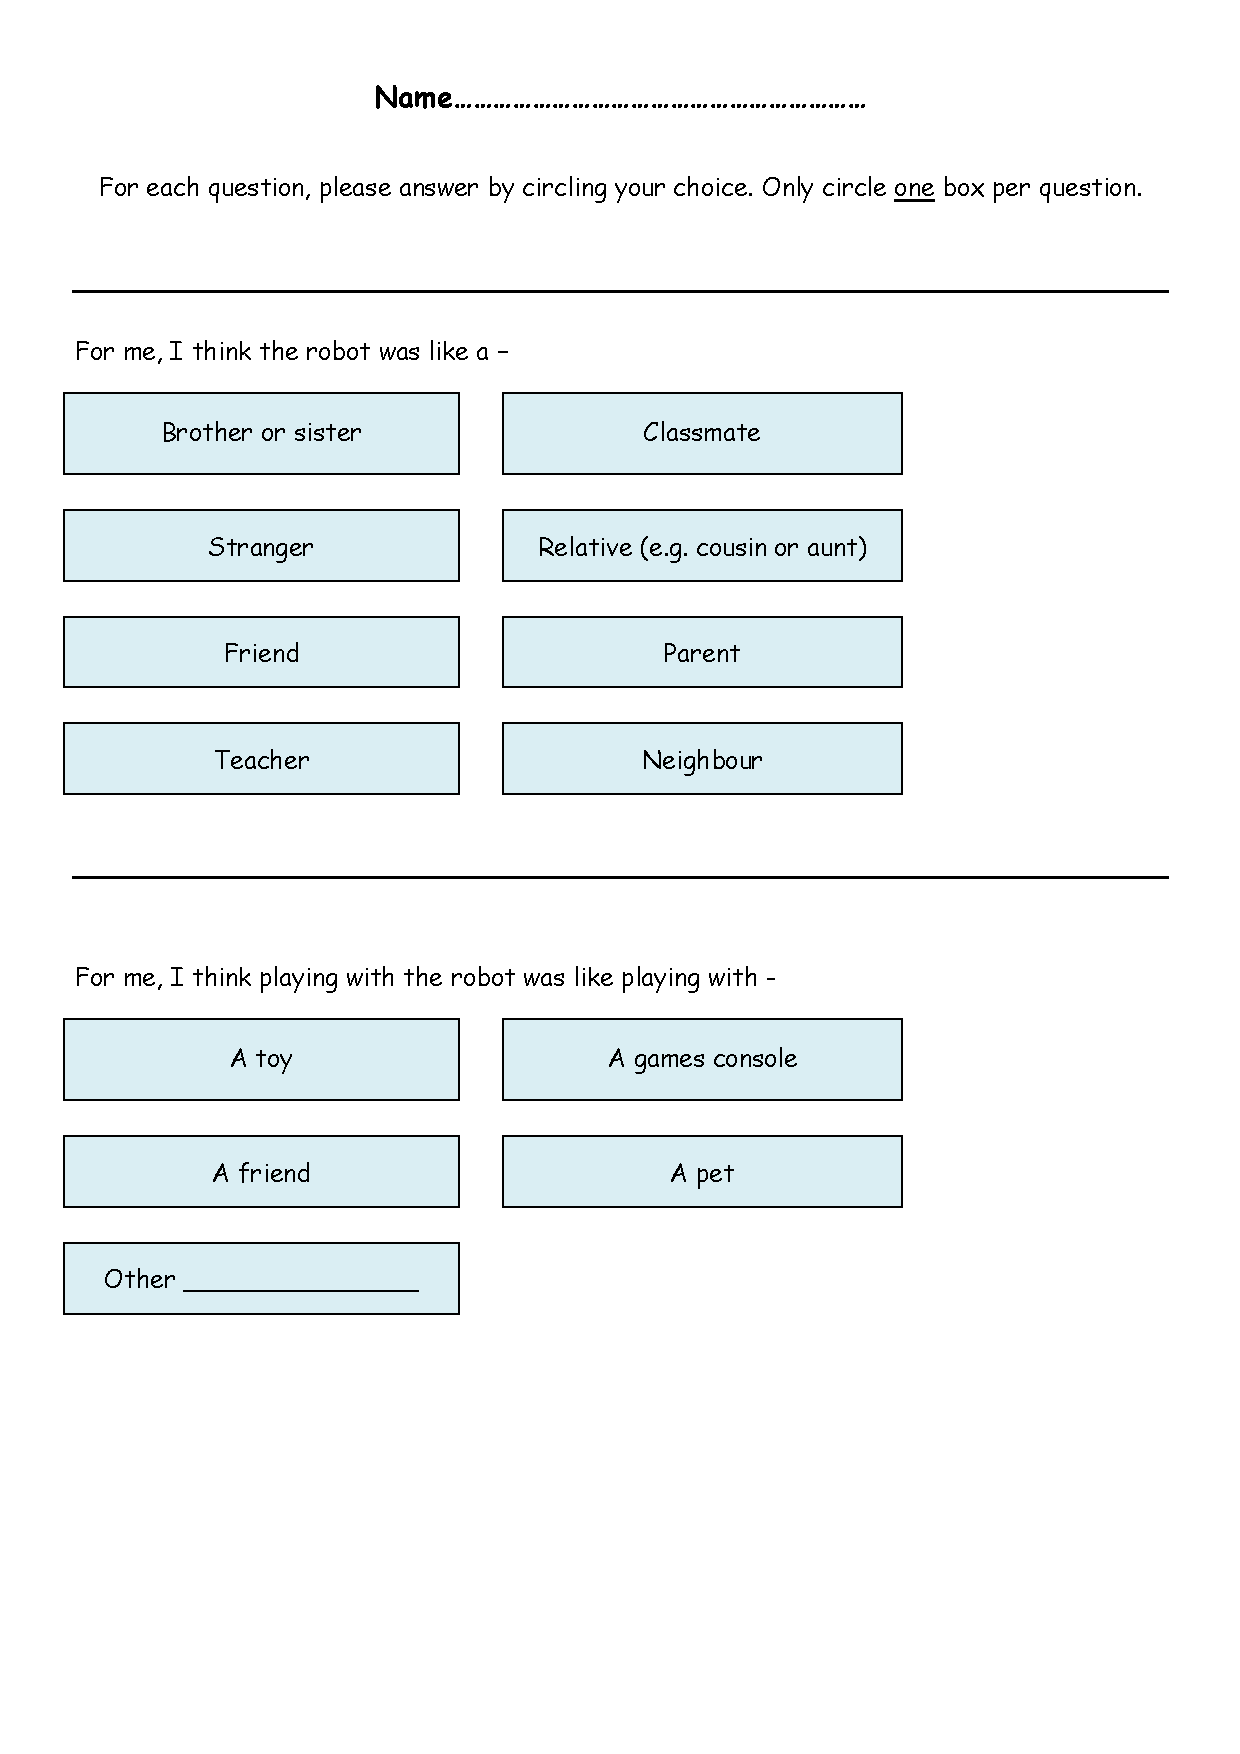
\includepdf[pages=1,pagecommand={},linktodoc=true]{appendices/RelationQuestionnaire.pdf}

\cleartooddpage
\chapter{Chapter \ref{chap:verbal} French Language Test} \label{app:frenchtest}
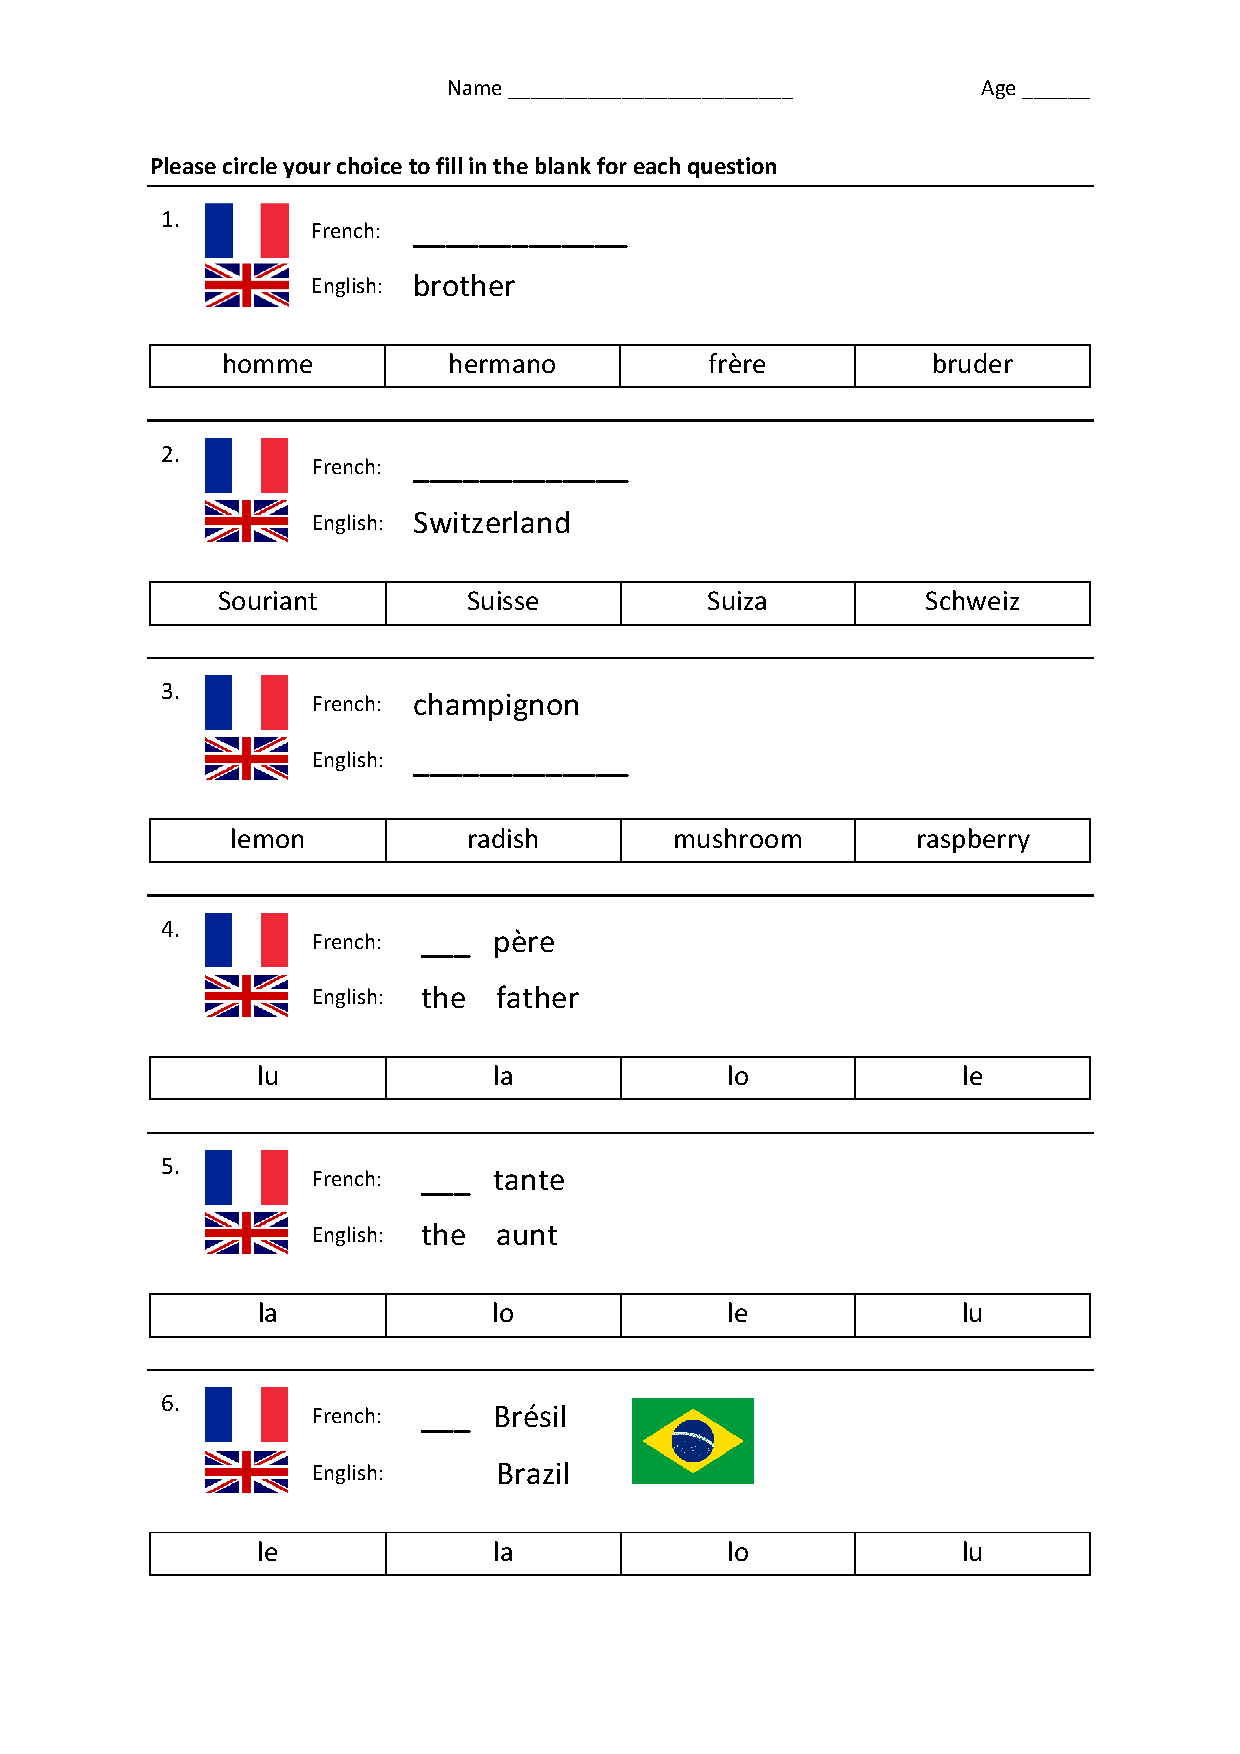
\includepdf[pages=1-2,pagecommand={},linktodoc=true]{appendices/FrenchTest.pdf}